\Exercise[number=6]
A source emits unstable particles, which decay at a distance \(x\) from
the source.
\begin{figure}[H]
    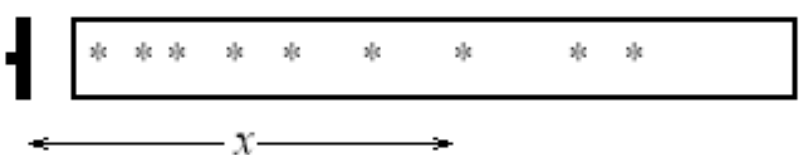
\includegraphics[scale=0.5]{B_6}
    \centering
\end{figure}
Quantity x is a real number that has an exponential distribution, with
characteristic distance \(\lambda\):
\[
    p(x|\lambda) \propto \exp{(-x/\lambda)}
\]
If \(N\) independent events \(\{ x_i, i = 1...N\}\) are observed, find an
expression for \(\lambda\). 
How does this expression change if you know that it must be
\(x > 1\) cm?

\Answer[number=6]
Let's define the dataset \(X=\{x_i|i=1...N\}\) and compute the normalization
factor \(K_{\lambda}\) by integration (notice that 0 is chosen instead
of \(-\infty\) as \(x\) is a distance and cannot be negative):
\begin{align*}
    \int_{0}^{+\infty}p(x|\mu)\,dx = 1 \Rightarrow
    \int_{0}^{+\infty}K_{\lambda}e^{-\frac{x}{\lambda}}\,dx
    =
    -K_{\lambda}\lambda\biggl[e^{-\frac{x}{\lambda}}\biggr]_{0}^{+\infty}
    =
    K_{\lambda}\lambda
    =
    1
    \Rightarrow
    K_{\lambda}
    =
    \frac{1}{\lambda}
\end{align*}
At this point, the likelihood and the log-likelihood can be written as
\[
    L(\lambda|X)=\prod_{i=1}^{N} \frac{1}{\lambda}e^{-\frac{x_i}{\lambda}}
    \Rightarrow
    \log{L(\lambda|X)}=-N\log{\lambda}-\frac{1}{\lambda}\sum_{i=1}^{N}x_i
\]
and the maximum likelihood estimator \(\hat{\lambda}\) is to be found by
deriving w.r.t. \(\lambda\) and setting the expression equal to 0:
\begin{align*}
    \frac{\partial{L(\lambda|X)}}{\partial{\lambda}}=0
    \Rightarrow
    -\frac{N}{\cancel{\lambda}}+\frac{1}{\lambda^{\cancel{2}}}\sum_{i=1}^{N}x_i=0
    \Rightarrow
    \hat{\lambda}=\frac{1}{N}\sum_{i=1}^{N}x_i
\end{align*}
\\
If \(x>1\) the lower integration bound is changed from 0 to 1, thus the
normalization factor is computed as follow:
\begin{align*}
    \int_{1}^{+\infty}p(x|\mu)\,dx = 1 \Rightarrow
    \int_{1}^{+\infty}K_{\lambda}e^{-\frac{x}{\lambda}}\,dx
    =
    -K_{\lambda}\lambda\biggl[e^{-\frac{x}{\lambda}}\biggr]_{1}^{+\infty}
    =
    K_{\lambda}\lambda e^{-\frac{1}{\lambda}}
    =
    1
    \Rightarrow
    K_{\lambda}
    =
    \frac{e^{\frac{1}{\lambda}}}{\lambda}
\end{align*}
Then, the likelihood and the log-likelihood are
\[
    L(\lambda|X)=\prod_{i=1}^{N} \frac{e^{\frac{1}{\lambda}}}{\lambda}e^{-\frac{x_i}{\lambda}}
    \Rightarrow
    \log{L(\lambda|X)}=\frac{N}{\lambda}-N\log{\lambda}-\frac{1}{\lambda}\sum_{i=1}^{N}x_i
\]
while the maximum likelihood estimator \(\hat{\lambda}\) is obtained by
deriving w.r.t. \(\lambda\) and setting the expression equal to 0:
\begin{align*}
    \frac{\partial{L(\lambda|X)}}{\partial{\lambda}}=0
    \Rightarrow
    -\frac{N}{\lambda^{\cancel{2}}}-\frac{N}{\cancel{\lambda}}+\frac{1}{\lambda^{\cancel{2}}}\sum_{i=1}^{N}x_i=0
    \Rightarrow
    -N-\lambda N+\sum_{i=1}^{N}x_i=0
    \Rightarrow
    \hat{\lambda}=\frac{1}{N}\sum_{i=1}^{N}x_i-1
\end{align*}